\documentclass[10pt,a4paper]{article}
\linespread{1.2}
\usepackage{verbatim}
\usepackage{geometry}
\usepackage{listings}
\usepackage{graphicx}


\geometry{right=2.0cm,left=2.0cm,top = 2.0cm, bottom = 2.0cm}

\lstdefinestyle{mystyle}{
    basicstyle=\ttfamily
}

\lstset{style=mystyle}

\title{CAAM 419/519, Homework \#4}
\author{\texttt{hc54}}
\date{December 8, 2022}

\begin{document}

\maketitle

\section{main.cpp script}
\subsection{Code part}
\begin{figure}[!ht]
        \centering 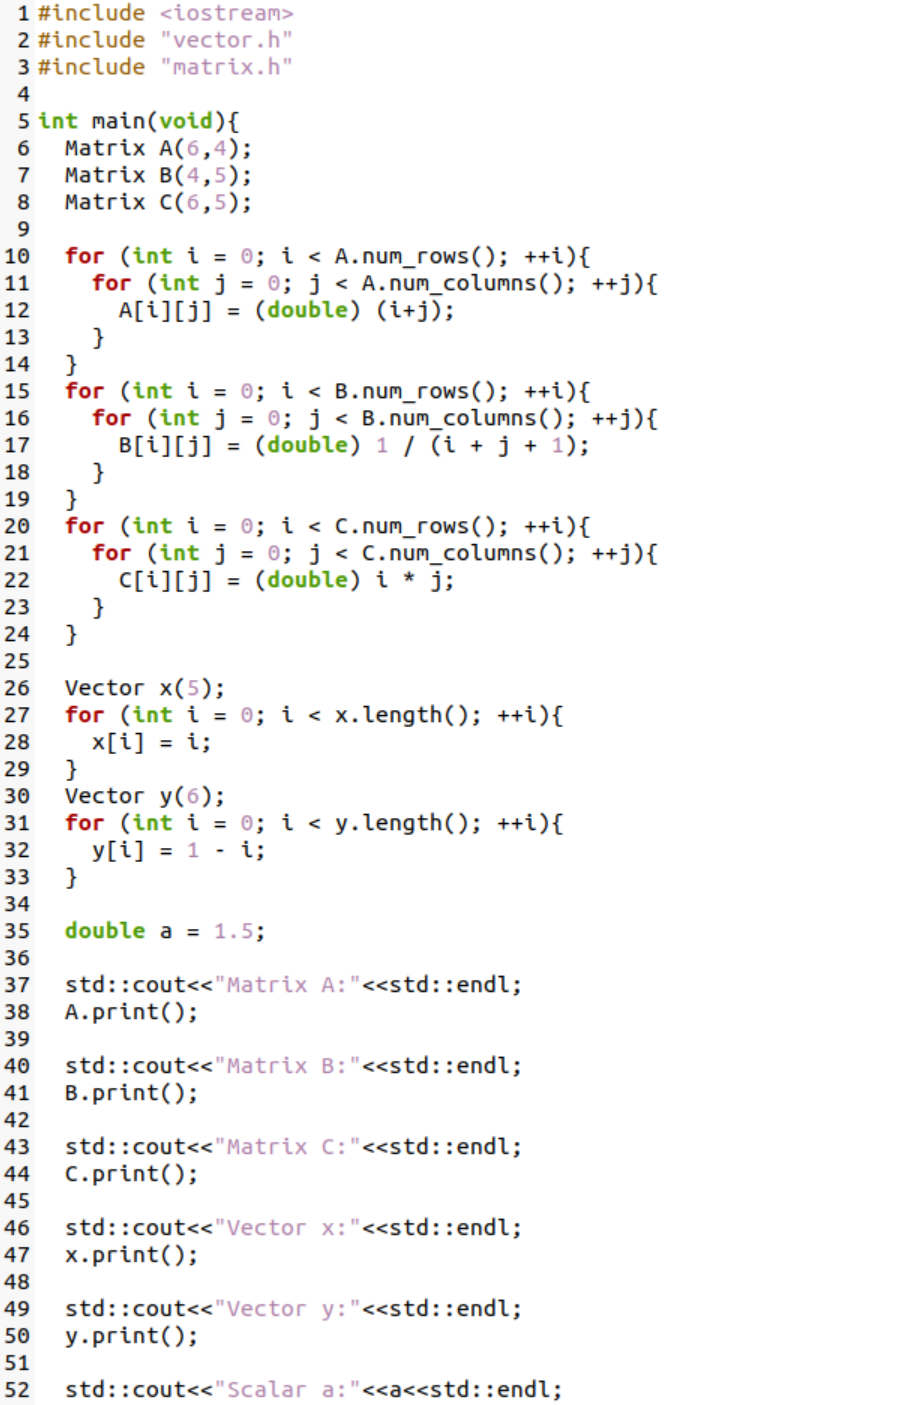
\includegraphics[scale=0.8]{figures/code1.png}
\end{figure}

\begin{figure}[!ht]
        \centering 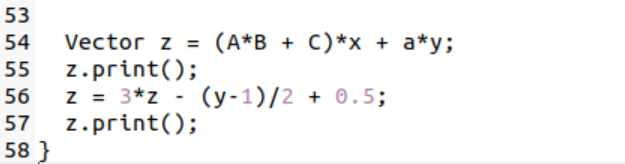
\includegraphics[scale=1]{figures/code2.png}
\end{figure}
\subsection{Output}
\begin{figure}[!ht]
        \centering 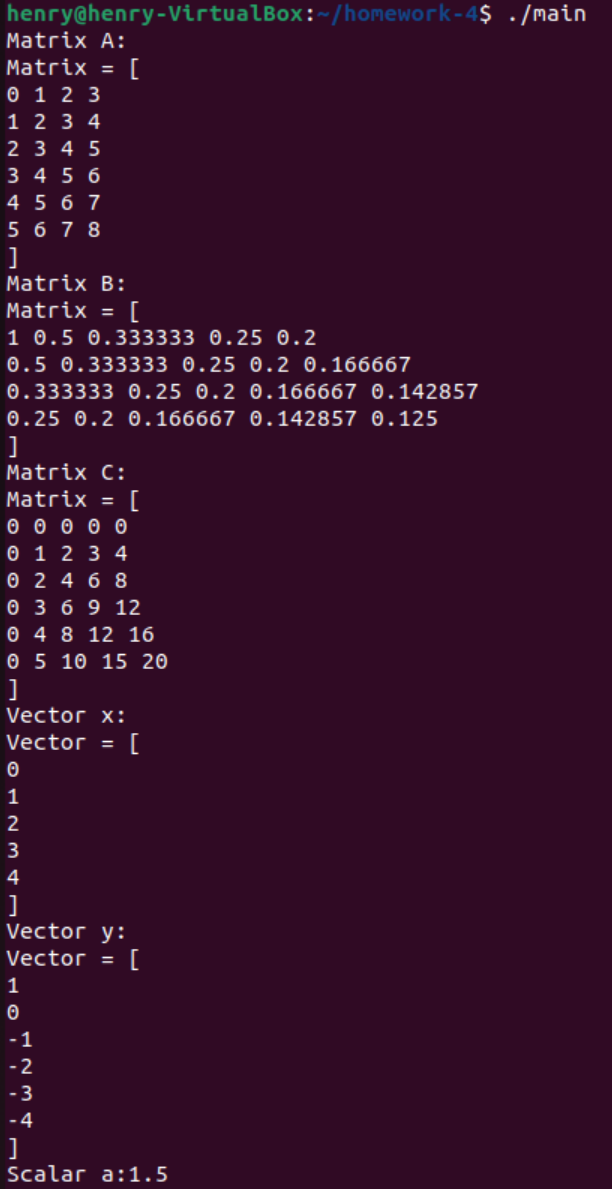
\includegraphics[scale=1]{figures/output1.png}
        \caption{Print of matrices, vectors, and scalar}
\end{figure}

\begin{figure}[!ht]
        \centering 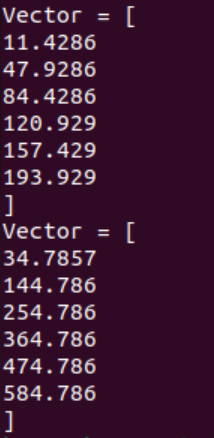
\includegraphics[scale=1]{figures/output2.png}
        \caption{Value of z computed}
\end{figure}

\section{Discussion}

When using x = x+y or x = x*y, we do an additional new vector or matrix to copy vector or matrix x. Therefore, we need to assign more memory. If we use *= or += operators, we can modify (*this) vector or matrix, which does not need additional memory and is more efficient. 

\end{document}
